\chapter{Anexo III - Manuales de usuario e Instalación}


En este anexo se proporcionarán los manuales de usuario e instalación de las herramientas necesarias para el desarrollo y la verificación del funcionamiento del \gls{tfm}. Además, se explicará el funcionamiento de los scripts de instalación generados, facilitando así el acceso a cualquier persona interesada en replicar los diferentes casos de uso. Los manuales de usuario detallarán los pasos necesarios para utilizar cada herramienta, incluyendo instrucciones de instalación, configuración y operación. Se proporcionarán ejemplos prácticos y se explicarán los conceptos clave relacionados con el uso de estas herramientas.\\
\\
Asimismo, se incluirá información sobre los scripts de instalación desarrollados, que permiten una instalación rápida y sencilla de las herramientas y componentes necesarios para reproducir los casos de uso del TFM. Estos scripts automatizan gran parte del proceso de instalación y configuración, lo que facilita a los usuarios la puesta en marcha de los entornos necesarios para el desarrollo y la evaluación.

%%%%%%%%%%%%%%%%%%%%%%%%%%%%%%%%%%%%%%%%%%%%%%%%%%%%%%%%%%%%%%%%%%%%%%%%%%%%%%%%%%%%%%%%%
\section{Herramienta \texttt{iproute2}}
\label{iproute2}
Se ha querido añadir esta sección, ya que la herramienta iproute2 va a ser fundamental a la hora de cargar los programas \gls{xdp} en el Kernel, consultar interfaces, o verificar en que \textit{Network namespace} se encuentra el usuario. Por todo lo anterior, la herramienta iproute2 será una de las piezas claves para gestión de las \textit{Network Namespaces}, y la verificación de los casos de uso.



\subsection{¿Qué es \texttt{iproute2?}}

Iproute2 es un paquete utilitario de herramientas para la gestión del \textit{Networking} en los sistemas Linux. Además, se encuentra ya en la mayoría de las distribuciones actuales. Sus desarrolladores principales son Alexey Kuznetsov y Stephen Hemminger, aunque hoy en día es un proyecto opensource donde cientos de personas contribuyen activamente en el repositorio\footnote{\url{https://github.com/shemminger/iproute2}}.  \\
\par
Actualmente, la versión más reciente de la herramienta es \texttt{v5.2.0}. Dicha versión será la que se utilizará en Ubuntu 18.04. El conjunto de utilidades que ofrece iproute2 está pensado para la sustitución de herramientas que se recogen en el paquete de \textbf{net-tools}, como por ejemplo a \texttt{ifconfig}, \texttt{route}, \texttt{netstat}, \texttt{arp}, etc. En la tabla \ref{tab:ipNettools} se pueden apreciar las herramientas de net-tools equivalentes en iproute2.

\begin{table}[ht]
    \centering
    \begin{tabular}{|c|c|}
        \hline
        \rowcolor[HTML]{C0C0C0}
        {\color[HTML]{000000} \textbf{net-tools}} & {\color[HTML]{000000} \textbf{iproute2}} \\ \hline
        \texttt{arp}                              & \texttt{ip neigh}                        \\ \hline
        \texttt{ifconfig}                         & \texttt{ip link}                         \\ \hline
        \texttt{ifconfig -a}                      & \texttt{ip addr}                         \\ \hline
        \texttt{iptunnel}                         & \texttt{ip tunnel}                       \\ \hline
        \texttt{route}                            & \texttt{ip route}                        \\ \hline
    \end{tabular}
    \caption{Comparativa de herramientas Iproute2 con paquete net-tools}
    \label{tab:ipNettools}
\end{table}

\subsection{¿Por qué necesitamos \texttt{iproute2}?}

Cuando se está trabajando con los programas XDP y se quiere comprobar su funcionamiento, se debe compilarlos. Esto se hará con los compiladores LLVM\footnote{\url{https://llvm.org/}} más clang\footnote{\url{https://clang.llvm.org/}}, como ya se comentaba en el estado del arte. Este proceso de compilación convertirá el código de los programas \gls{xdp}, en un \textit{bytecode} \gls{bpf}, y más tarde, se almacenará este \textit{bytecode} en un fichero de tipo \gls{elf}. Una vez compilados, se tendrá que anclarlos en el Kernel, y es  en este punto es donde entrará iproute2, ya que tiene un cargador \gls{elf} ( generalmente se trabajará con extensiones del tipo *.o ). \newline
\newline
Además, la herramienta iproute2 permite al usuario comprobar si una interfaz tiene cargado un programa \gls{xdp}. Arrojando en dicho caso, el identificador del programa \gls{xdp}, que tiene anclado la interfaz y si este programa está cargado de una forma nativa o de una forma genérica. Al final de la esta sección, se indicará cómo hacer esta comprobación.

\subsection{Estudio de compatibilidad de la herramienta \texttt{iproute2} en Ubuntu}

Al trabajar con esta herramienta para cargar programas XDP, se necesita  la versión que soporte el cargador ficheros \gls{elf}. Si usted tiene la versión de iproute2 que viene instalada por defecto en Ubuntu 16.04, le indicamos que aún no da soporte a \gls{xdp}. Inicialmente se buscó información relativa a partir de que versión se daba soporte a \gls{xdp} tanto en Ubuntu 16.04, como en Ubuntu 18.04. Como no se encontró información precisa sobre ello, se ha realizado un estudio de la compatibilidad de iproute2 a través de Ubuntu 16.04 y Ubuntu 18.04.\\
\par

Este estudio de compatibilidad se llevó a cabo descargando cada versión de iproute2, compilándola, e instalándola en nuestra máquina. Por último, para verificar si dicha versión daba soporte a \gls{xdp}, se comprobaba si un programa \gls{xdp} genérico que se sabía que funcionaba, cargaba o no, y si éste mostraba estadísticas sobre su carga. Más adelante, se indicará cómo compilar e instalar una versión en particular de iproute2.  \\
\par

Como se puede apreciar en la siguiente tabla \ref{tab:iproute}, en Ubuntu 16.04 a partir de la versión \texttt{v4.14.0} no existe compatibilidad. Esto es debido a que requiere librerías de enlazado extensible de formato (No \gls{elf} Support). Para resolver este requerimiento se debería añadir una versión más reciente de la librería \textbf{libelf\_dev}. Se puede agregar dicha librería, pero al hacerlo aparecerán dependencias que se van ramificando una a una llegando a librerías más sensibles para nuestro sistema como \textbf{libc6}, por lo que se decidió no comprobar el funcionamiento añadiendo las nuevas librerías requeridas para no comprometer el sistema.


\begin{table}[ht]
    \centering
    \resizebox{\textwidth}{!}{%
        \begin{tabular}{|l|c|c|c|c|c|c|c|c|c|c|c|c|c|}
            \hline
            {\color[HTML]{333333} \textbf{Versiones IProute2}} & \multicolumn{1}{l|}{\cellcolor[HTML]{6A8AE5}v4.9.0}        & \multicolumn{1}{l|}{\cellcolor[HTML]{6A8AE5}v4.10.0}       & \multicolumn{1}{l|}{\cellcolor[HTML]{6A8AE5}v4.11.0}       & \multicolumn{1}{l|}{\cellcolor[HTML]{6A8AE5}v4.12.0} & \multicolumn{1}{l|}{\cellcolor[HTML]{6A8AE5}v4.13.0} & \multicolumn{1}{l|}{\cellcolor[HTML]{6A8AE5}v4.14.0} & \multicolumn{1}{l|}{\cellcolor[HTML]{6A8AE5}v4.15.0} & \multicolumn{1}{l|}{\cellcolor[HTML]{6A8AE5}v4.16.0} & \multicolumn{1}{l|}{\cellcolor[HTML]{6A8AE5}v4.17.0} & \multicolumn{1}{l|}{\cellcolor[HTML]{6A8AE5}v4.18.0} & \multicolumn{1}{l|}{\cellcolor[HTML]{6A8AE5}v4.20.0} & \multicolumn{1}{l|}{\cellcolor[HTML]{6A8AE5}v5.1.0} & \multicolumn{1}{l|}{\cellcolor[HTML]{6A8AE5}v5.2.0} \\ \hline
            \rowcolor[HTML]{FD6864}
            \cellcolor[HTML]{FFC702}Ubuntu 16.04               & \cellcolor[HTML]{67FD9A}{\color[HTML]{6665CD} No XDP supp} & \cellcolor[HTML]{67FD9A}{\color[HTML]{6665CD} No XDP supp} & \cellcolor[HTML]{67FD9A}{\color[HTML]{6665CD} No XDP supp} & \cellcolor[HTML]{67FD9A}{\color[HTML]{036400} Si}    & \cellcolor[HTML]{67FD9A}{\color[HTML]{036400} Si}    & {\color[HTML]{9A0000} No}                            & {\color[HTML]{9A0000} No}                            & {\color[HTML]{9A0000} No}                            & {\color[HTML]{9A0000} No}                            & {\color[HTML]{9A0000} No}                            & {\color[HTML]{9A0000} No}                            & {\color[HTML]{9A0000} No}                           & {\color[HTML]{9A0000} No}                           \\ \hline
            \cellcolor[HTML]{9870D0}Ubuntu 18.04               & -                                                          & -                                                          & -                                                          & -                                                    & -                                                    & -                                                    & \cellcolor[HTML]{67FD9A}{\color[HTML]{036400} Si}    & \cellcolor[HTML]{67FD9A}{\color[HTML]{036400} Si}    & \cellcolor[HTML]{67FD9A}{\color[HTML]{036400} Si}    & \cellcolor[HTML]{67FD9A}{\color[HTML]{036400} Si}    & \cellcolor[HTML]{67FD9A}{\color[HTML]{036400} Si}    & \cellcolor[HTML]{67FD9A}{\color[HTML]{036400} Si}   & \cellcolor[HTML]{67FD9A}{\color[HTML]{036400} Si}   \\ \hline
        \end{tabular}%
    }
    \caption{Estudio de compatibilidad de la herramienta Iproute2}
    \label{tab:iproute}
\end{table}

\begin{figure}
    \centering
    \begin{tikzpicture}[node distance=2cm, auto]
        % Cuadros
        \node (deps) [rectvioleta,text width=3cm] {\texttt{libelf\_dev} \par};
        \node (deps2) [rectvioleta,below of=deps,text width=3cm] { \texttt{libelf1} \par};
        \node (deps3) [rectvioleta,right of=deps2,xshift=3cm, text width=3cm] { \texttt{zliblg} \par};
        \node (harddep) [rectnaranja,below of=deps2,text width=3cm]{ \texttt{libc6} \par};
        % Flechas
        \draw[arrow] (deps) -- (deps2);
        \draw[arrow] (deps2) -- (deps3);
        \draw[arrow] (deps2) -- (harddep);

    \end{tikzpicture}
    \caption{Ramificación de dependencias de Iproute2.}
    \label{fig:DependenciasIproute}
\end{figure}

\newpage

\subsection{Compilación e instalación de \texttt{iproute2}}
El proceso es prácticamente análogo tanto en Ubuntu 16.04 como en Ubuntu 18.04, salvo por una única diferencia que se indicará más adelante. Ahora se mostrarán los pasos necesarios para la compilación e instalación de una versión, en concreto de la herramienta iproute2.

\begin{itemize}
    \item En primer lugar, se necesitará de instalar los paquetes necesarios para la configuración previa a la compilación.
          \begin{itemize}
              \item \texttt{bison}, es un herramienta generadora de analizadores sintácticos de propósito general.
              \item \texttt{flex}, es una herramienta para generar programas que reconocen patrones léxicos en el texto.
              \item \texttt{libmnl-dev}, es una librería de espacio de usuario orientada a los desarrolladores de Netlink. Netlink\footnote{\url{https://www.man7.org/linux/man-pages/man7/netlink.7.html}} es una interfaz entre espacio de usuario y espacio de Kernel vía sockets.

              \item \texttt{libdb5.3-dev}, éste es un paquete de desarrollo que contiene los archivos de cabecera y librerías estáticas necesarias para la BBDD de Berkley (\textit{Key/Value}).

              \item Se entiende que se tiene el paquete \texttt{wget}. En caso de no tenerlo, solo se deberá añadir para poder descargar la herramienta.
          \end{itemize}
\end{itemize}
\begin{lstlisting}[language= bash, style=Consola2, caption={Instalación de las dependencias de Iproute2},label=code:iproute2_deps]
   sudo apt-get install bison flex libmnl-dev libdb5.3-dev
\end{lstlisting}
\begin{itemize}
    \item En segundo lugar, se debe descargar el comprimido de la herramienta iproute2. Al haber varios paquetes, se descargará aquel cuya versión sea con la que se quiere trabajar. Podemos descargarlas desde aquí: \href{https://mirrors.edge.kernel.org/pub/linux/utils/net/iproute2/}{\textbf{kernel.org}}.
\end{itemize}
\begin{lstlisting}[language= bash, style=Consola, caption={Obtención del source de Iproute2},label=code:iproute2_src]
   wget -c http://ftp.iij.ad.jp/pub/linux/kernel/linux/utils/net/iproute2/iproute2-4.15.0.tar.gz
\end{lstlisting}

\begin{itemize}
    \item En tercer lugar, se debe descomprimir el comprimido de la herramienta. Acto seguido, se procederá a configurarla, compilarla e instalarla.
\end{itemize}

\begin{lstlisting}[language= bash, style=Consola, caption={Compilación e instalación de Iproute2},label=code:iproute2_install]
   # Se descomprime y se entra al directorio
   tar -xvfz $(tar).tar.gz && cd $tar
   
   # Se configura
   ./configura
   
   # Se compila e instala, para añadir el nuevo binario en el path
   sudo make
   sudo make install
\end{lstlisting}
\subsubsection{Diferencias con Ubuntu 18.04}

La única diferencia en el proceso de instalación de la herramienta de iproute2 en Ubuntu 18.04, es añadir un paquete extra antes de proceder a configurar, compilar e instalar. El paquete extra es \textbf{pkg-config}; de no añadirlo fallará al lanzar el script de configuración y hacer el build.
\begin{lstlisting}[language= bash, style=Consola, caption={Instalación de las dependencias de Iproute2 - Ubuntu 18.04},label=code:iproute2_deps18]
    sudo apt-get install bison flex libmnl-dev libdb5.3-dev pkg-config
\end{lstlisting}

\subsection{Comandos útiles con \texttt{iproute2}}

A continuación, se indican los comandos más frecuentes con la herramienta iproute2. Todos ellos han sido utilizados en el proceso de desarrollo del proyecto y en el proceso de verificación de los distintos casos de uso. Por ello, se considera que este apartado puede ser de gran utilidad para el lector que nunca ha trabajado con esta herramienta.

\begin{lstlisting}[language= bash, style=Consola, caption={Comandos útiles con iproute2},label=code:iproute2_use]
    # Listar interfaces y ver direcciones asignadas
    ip addr show
    
    # Poner/Quitar dirección a una interfaz
    ip addr add {IP} dev {interfaz}
    ip addr del {IP} dev {interfaz}
    
    # Levantar/deshabilitar una interfaz 
    ip link set {interfaz} up/down
    
    # Listar rutas
    ip route list 
    
    # Obtener ruta para una determinada dirección IP
    ip route get {IP}
    
    # Listar Network namespace con nombre
    ip netns list
    

\end{lstlisting}
\newpage
%%%%%%%%%%%%%%%%%%%%%%%%%%%%%%%%%%%%%%%%%%%%%%%%%%%%%%%%%%%%%%%%%%%%%%%%%%%%%%%%%%%%%%%%%%%%%%%%%%

\section{Herramienta \texttt{tcpdump}}
\label{tcpdump}

La inclusión de esta sección se motiva por proporcionar un punto de referencia para aquellos usuarios que no están familiarizados con tcpdump. A lo largo de todas las secciones del proyecto, se utilizará esta herramienta para verificar el correcto funcionamiento de los casos de uso. El objetivo de esta sección es ofrecer una guía práctica sobre cómo utilizar tcpdump, especialmente dirigida a aquellos usuarios que no tienen experiencia previa con la herramienta. Se proporcionarán instrucciones detalladas sobre cómo instalar y ejecutar tcpdump, así como ejemplos de comandos comunes para capturar y analizar el tráfico de red.\\
\\
Al comprender cómo utilizar tcpdump, los usuarios podrán verificar de manera efectiva si los casos de uso implementados en el proyecto están funcionando según lo esperado. Esta herramienta les permitirá examinar el tráfico de red en tiempo real y obtener información relevante para la evaluación y solución de problemas.

\subsection{¿Qué es \texttt{tcpdump}?}

Tcpdump es un analizador de tráfico diseñado para inspeccionar los paquetes entrantes y salientes de una interfaz. La peculiaridad de esta herramienta es que funciona mediante línea de comandos y tiene soporte en la mayoría de los sistemas UNIX\footnote{Unix es un sistema operativo desarrollado en 1969 por un grupo de empleados de los laboratorios Bell}, como Linux, macOS y OpenWrt. La herramienta está escrita en lenguaje C, lo que le confiere un alto rendimiento, y utiliza libpcap\footnote{\url{https://github.com/the-tcpdump-group/libpcap}} para la captura de paquetes.\\
\\
Fue desarrollada en 1988 por trabajadores de los laboratorios de Berkeley. En la actualidad, cuenta con una gran comunidad de desarrolladores respaldándola en su repositorio oficial\footnote{\url{https://github.com/the-tcpdump-group/tcpdump}}, donde se lanzan periódicamente nuevas actualizaciones (última versión \texttt{v4.99.4}).

\subsection{¿Por qué necesitamos \texttt{tcpdump}?}

En la actualidad, es común desarrollar en entornos distribuidos, utilizando contenedores o máquinas virtuales para delimitar el entorno de desarrollo. Por esta razón, se trabaja de forma remota, conectándose a la máquina o contenedor mediante el protocolo SSH\footnote{\url{https://www.ssh.com/ssh/}}.\\
\\
Esto conlleva numerosas ventajas, pero también puede presentar complicaciones. Por ejemplo, si alguien no sabe cómo configurar un \textit{X Server} para ejecutar aplicaciones gráficas de forma remota, no podría utilizar herramientas como Wireshark. En este sentido, tcpdump resulta especialmente útil, ya que no requiere ninguna configuración adicional para ejecutarse de forma remota. Además, su rápido inicio, en comparación con otros ``sniffers" como Wireshark, ha convertido a tcpdump en una herramienta fundamental para verificar casos de uso.

\subsection{Instalación de \texttt{tcpdump}}

Como se mencionó anteriormente, tcpdump cuenta con un amplio soporte en sistemas UNIX, por lo que suele estar preinstalado en la mayoría de las distribuciones Linux. Sin embargo, en caso de no tenerlo instalado, es posible instalarlo fácilmente siguiendo los pasos que se muestran a continuación (Ver bloque \ref{code:tcpdump}). Estos comandos actualizarán los repositorios de paquetes y descargarán e instalarán tcpdump en el sistema. Una vez completada la instalación, tcpdump estará listo para su uso.

\begin{lstlisting}[language= bash, style=Consola2, caption={Instalación del paquete Tcpdump},label=code:tcpdump]
    sudo apt install -y tcpdump
\end{lstlisting}

\subsection{Comandos útiles con \texttt{tcpdump}}


A continuación, se presentan algunos comandos comunes que se han utilizado durante el proceso de verificación de los casos de uso con la herramienta tcpdump. Estos comandos han sido seleccionados debido a su relevancia y utilidad, y se considera que pueden ser de gran ayuda para aquellos lectores que no estén familiarizados con esta herramienta. No obstante, se recomienda encarecidamente que el lector consulte la página de manual de tcpdump\footnote{\url{https://linux.die.net/man/8/tcpdump}} para obtener información más detallada sobre el uso básico de tcpdump y explorar todas sus capacidades. Estos son solo algunos ejemplos de los comandos más utilizados con tcpdump. Como se mencionó anteriormente, se recomienda encarecidamente al lector que consulte la página de manual de tcpdump para obtener una comprensión más completa de sus capacidades y explorar otros filtros y opciones disponibles.

\begin{lstlisting}[language= bash, style=Consola2, caption={Comandos útiles con Tcpdump},label=code:tcpdump_use]
    # Indicar sobre que Interfaz se quiere sniffear
    tcpdump -i {Interfaz}
    
    # Podemos almacenar la traza a un archivo para su posterior análisis
    tcpdump -w fichero.pcap -i {Interfaz}
    
    # También podemos ver una traza desde un archivo
    tcpdump -r fichero.pcap
    
    # Podemos filtrar por  puerto
    tcpdump -i {Interfaz} port {Puerto}
    
    # Podemos filtrar por  dirección IP destino/origen
    tcpdump -i {Interfaz} dst/src {IP}
    
    # Podemos filtrar por protocolo
    tcpdump -i {Interfaz} {protocolo}
    
    # Listar interfaces disponibles para escuchar de ellas 
    tcpdump -D
    
     # Limitar el número de paquetes a sniffear
    tcpdump -i {Interfaz} -c {Número de paquetes}
\end{lstlisting}
\vspace{1cm}
\begin{figure}[ht]
    \centering
    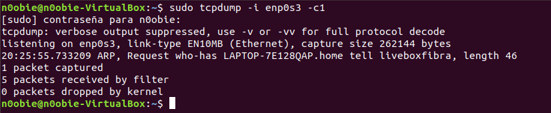
\includegraphics[width=\textwidth]{archivos/img/anexos/tcpdump_cli_edited.png}
    \caption{Interfaz de tipo CLI de Tcpdump}
    \label{tcpdumpCli}
\end{figure}

%%%%%%%%%%%%%%%%%%%%%%%%%%%%%%%%%%%%%%%%%%%%%%%%%%%%%%%%%%%%%%%%%%%%%%%%%%%%%%%%%%%%%%%%%%%%%%%%%%
\newpage
\section{Herramienta Mininet}
\label{sec:ToolsMininet}
La motivación de añadir esta sección es la de poder indicar al lector como se ha instalado la herramienta de Mininet en las distintas máquinas descritas en el pliego de condiciones (Anexo \ref{ch:anexoPliegoCondiciones}). Todo el proceso de instalación se ha llevado acabo en una máquina Linux, con las especificaciones indicadas en la siguiente tabla (Tabla \ref{tab:ToolsMininet}).

\begin{table}[ht!]
    \centering
    \resizebox{0.6\columnwidth}{!}{%
        \begin{tabular}{|c|c|c|c|}
            \hline
            \rowcolor[HTML]{EFEFEF}
            \textbf{Distribución Linux} & \textbf{Cores} & \textbf{Memoria} & \textbf{Disco} \\ \hline
            Ubuntu 22.04 LTS            & 2              & 4096 MiB         & 40 GiB         \\ \hline
        \end{tabular}%
    }
    \caption{Especificaciones máquina de instalación Mininet}
    \label{tab:ToolsMininet}
\end{table}

Para la instalación necesitaremos de conectividad a Internet y de la herramienta \texttt{git} para clonar el repositorio de \texttt{Mininet}. En caso de no tener la herramienta de \texttt{git}, podremos instalarla ejecutando el comando del bloque de código \ref{code:git_install}.

\begin{lstlisting}[language= bash, style=Consola2, caption={Instalación de la herramienta git},label=code:git_install]
    # El parametro -y se indica para confirmar la instalación de la herramienta
    sudo apt install -y git 
\end{lstlisting}
\vspace{1cm}

Una vez disponemos de la herramienta \texttt{git} para clonar el repositorio de \texttt{Mininet}, vamos a clonarlo, y lanzar el script de instalación que incorpora junto al source para instalar la herramineta. A continuación, en el bloque de código \ref{code:Mininet_install} se indica los comandos ejecutados para instalar la herrmaienta de \texttt{Mininet}.


\begin{lstlisting}[language= bash, style=Consola2, caption={Instalación de la herramienta Mininet},label=code:Mininet_install]
    # Clonamos el repositorio de Mininet
    git clone https://github.com/davidcawork/mininet.git

    # Accedemos al directorio
    cd mininet

    # Lanzamos el script de instalación (Openflow 1.3 - Ryu - Wireshark dissector)
    sudo util/install.sh -3fmnyv
\end{lstlisting}
\vspace{1cm}


%%%%%%%%%%%%%%%%%%%%%%%%%%%%%%%%%%%%%%%%%%%%%%%%%%%%%%%%%%%%%%%%%%%%%%%%%%%%%%%%%%%%%%%%%%%%%%%%%%